\section{Exploratory Study 2}
\label{sec:ch3-study2}
We conducted a building walk to explore how occupants experience and interpret smart environments over time. Framed through an AfI lens, we focused on how bodily, spatial, and social cues shape sense-making. Below, we outline the methodology and analysis, followed by our thematic findings.

\subsection{Building Walk}
\label{subsec:ch3-s2-methodology}
The building walk was designed as a semi-structured, participant-led conversation~\cite{mitchell2020no} to elicit nuanced, subjective accounts of experience in smart building spaces. Building blueprints were used to collaboratively plan a walking route through three spaces chosen by the participants.\sidenote{Our pilot study found that visiting four or more spaces reduced reflection quality and increased fatigue.} This selection helped situate the walk in participants’ own routines and preferences. To guide conversations, we prepared semi-structured prompts around six topics: \textit{usage}, \textit{technology}, \textit{emotion}, \textit{comfort}, \textit{experience}, and \textit{satisfaction}. These were adapted from prior smart building studies~\cite{margariti2021understanding, mitchell2020no} and refined by the five categories from Study 1 (c.f. ~\autoref{sec:ch3-s1-findings}). At each space, participants selected a prompt to initiate dialogue, with the session moderated by the first author.

Each session also included a \textbf{body mapping} activity, where participants used a printed outline of the human body to mark, annotate, or sketch how they were experiencing the space~\cite{turmo2023towards} (see supplementary materials). These body maps served as \textit{reflective artefacts}, supporting inward attention and awareness. While not part of our analysis, these were meant to help participants tune into their bodily experience.

\begin{mainfigure}[tbp]
  \begin{subfigure}[t]{.48\linewidth}
    \centering
    \includegraphics[width=\linewidth,height=4.15cm]{images/study_2/setup.jpg}
    \caption{The building walk setup for participants.}
    \label{fig:bw-setup}
  \end{subfigure}
  \hfill
  \begin{subfigure}[t]{.48\linewidth}
    \centering
    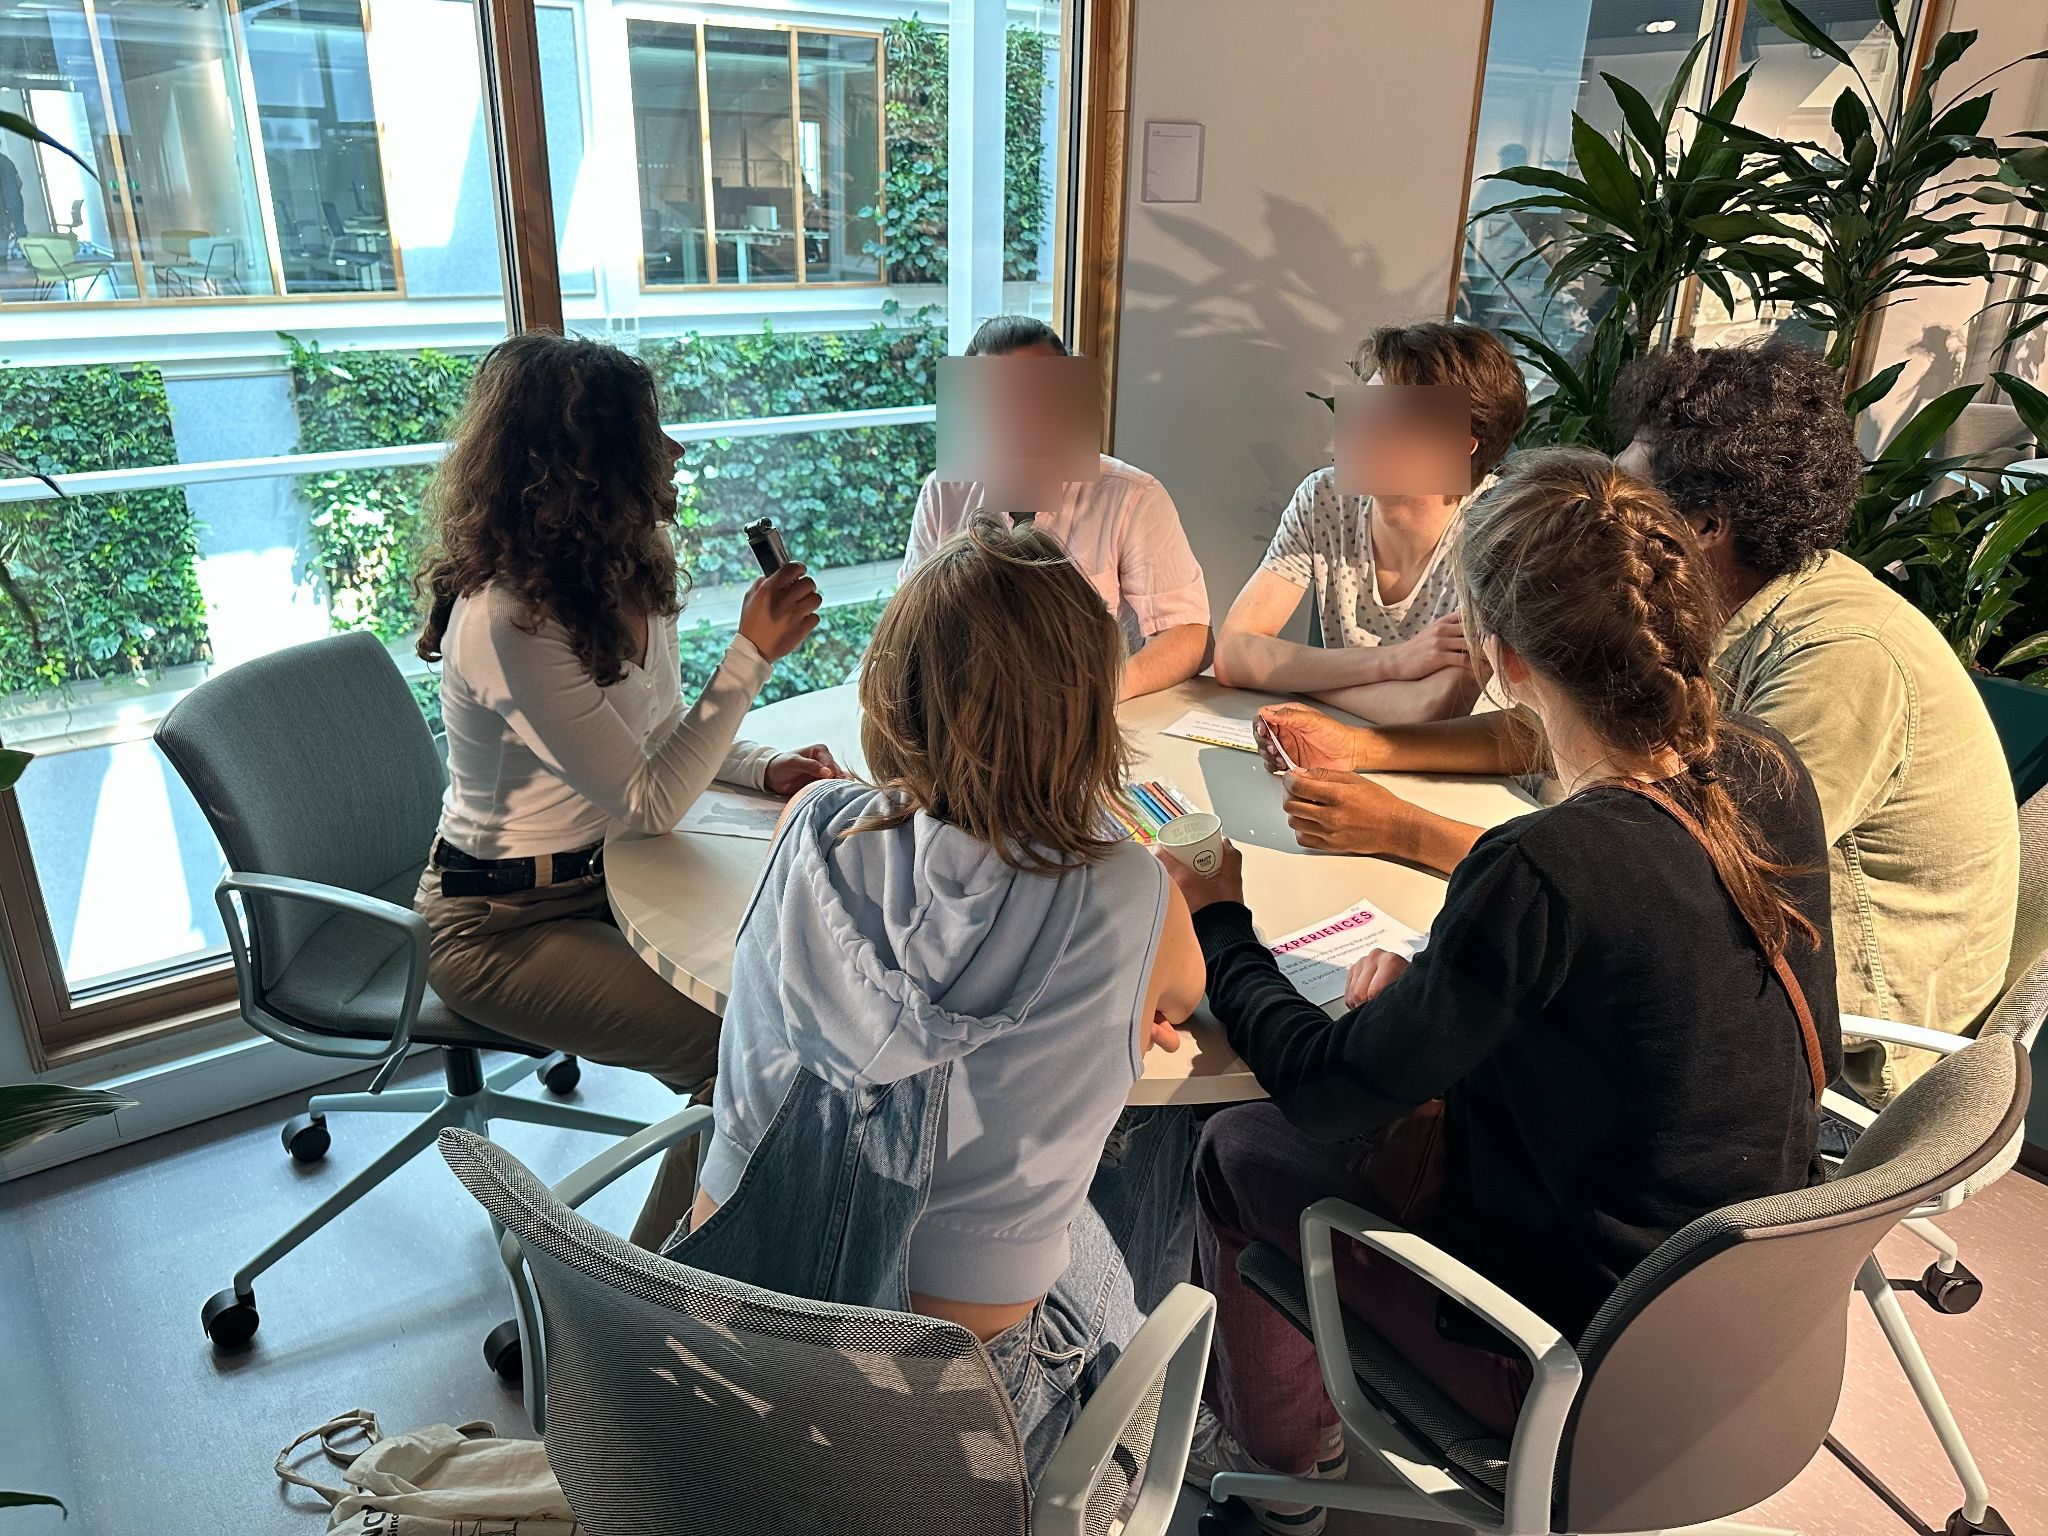
\includegraphics[width=\linewidth]{images/study_2/walk.jpg}
    \caption{A session with participants engaging in a conversation moderated by the researcher.}
    \label{fig:bw-session}
  \end{subfigure}

  \caption{An overview of the building walk: (a) setup from a session including informed consent and demographic forms, blueprints, question prompts, and body maps; and (b) a session underway at a group work space.}
  \label{fig:s2-overview}
  \Description{Two photographs documenting the building walk study. (a) A table setup showing printed informed consent and demographic forms, building floor plans, question prompt cards, and body-mapping templates prepared for participants. (b) A study session in progress, showing participants and a researcher standing and talking together in a shared indoor workspace during the building walk.}
\end{mainfigure}


\paragraph{Study Procedure}
\label{subsec:ch3-s2-procedure}
The building walk study comprised: a pre-walk introduction, the walk, and a post-walk reflection. First, participants reviewed study information and materials and signed consent forms. Next, they selected three indoor spaces to visit. During the walk, groups visited each space where they completed the body mapping exercise and conversed for 30 minutes. Post-walk, participants collectively and individual reflected on their body maps (\autoref{fig:s2-overview}). Each session was 75 to 90 minutes and was audio-recorded.


\paragraph{Participants}
\label{subsec:ch3-s2-participants}
We recruited $14$ participants ($8$F, $6$M) across three group sessions of 4–5 people. All were university students ($M_{\text{age}} = 22.2$, $SD = 2.08$) who used the building at least once per week. Recruitment took place via survey sign-ups and building posters, and participants received a €15 gift card.


\begin{mainfigure}[tbp]
    \centering
    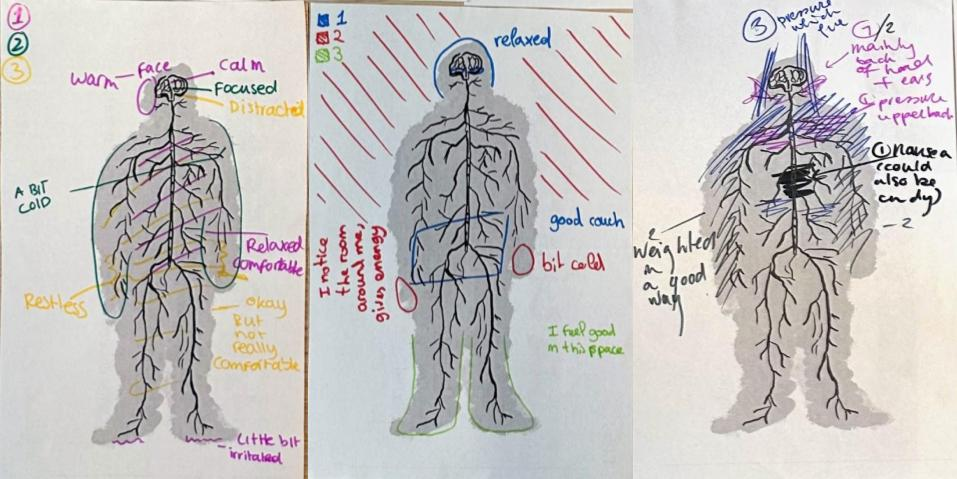
\includegraphics[width=\linewidth]{images/study_2/bodymaps-sample.jpg}
    \caption{Some examples of body maps that were used as reflective artefacts during the building walk, allowing participants to ``turn inwards'' and express sensations and emotions that may have otherwise remain unspoken. Participants were invited to annotate the maps throughout the session, marking bodily responses across different spaces.}
    \label{fig:s2-bodymaps}
    \Description{Photograph showing multiple annotated body map templates used in the study. Each body map depicts a simplified human silhouette with handwritten notes, marks, and symbols indicating bodily sensations or feelings. The annotations appear in different areas of the body outlines, reflecting participants’ responses recorded during the building walk across different spaces.}
\end{mainfigure}

\subsection{Methodology and Data Analysis}
\label{subsec:ch3-s2-analysis}
We collected approximately four hours of audio-recorded dialogue, $14$ annotated body maps, and marked-up building blueprints. All data was digitised, transcribed, and anonymised prior to analysis. We analysed the building walk conversations using a reflexive thematic analysis~\cite{braun2023thematic} suited for examining patterns of meaning in qualitative data---especially in under-explored domains~\cite{clarke2013successful, braun2013shouldn}. This involved an open, iterative coding process of semantic and latent meanings. Initial familiarisation with the transcripts was followed by line-by-line coding, resulting in over 420 codes (e.g. \textit{``Spatial quality of environment indicates type of work''},  ``Smart technology means invisibility'' ). Codes were then collated into 10 preliminary themes, which were iteratively refined into five final themes. Body maps were used to help participants externalise their experiences, and therefore not analysed (examples in \autoref{fig:s2-bodymaps}). The analysis was led by the first author together with the third author. Both authors reviewed the data but the first author led the development of themes that were refined through repeated readings and discussions between the authors.



\subsection{Building Walk Findings}
\label{sec:ch3-s2-findings}
To examine how occupants make sense of smart building experiences, we now present five themes, developed using ~\citet{braun2023thematic}'s reflexive thematic analysis. These trace the \textbf{W}ays in which architectural spaces are experienced (summarised in \autoref{tab:afi-theme-overview}).


\paragraph{W1 --- Interpreting the Somatic Experience Over Time}
\label{theme:w1}

Occupants often read their own bodily sensations~\cite{hook2018designing} as real-time feedback that shaped how they interpreted the space, adapted their behaviour, and ultimately decided whether to stay. These impressions unfolded across different tempos and levels of clarity. We observed four recurring patterns in how participants sensed and interpreted their bodily responses. 

Some sensations were instant and decisive (``yes'' or ``no'') prompting quick action: \textit{``I stepped in and the light\ldots.instantly felt, nope---not going to be able to focus here.''} Such cues often led to immediate acceptance or rejection of a space. Other sensations were subtle, peripheral, and hard to name, but still shaped the experience: \textit{``It’s not bad, I guess\ldots I just don’t feel like settling in here for some reason.''}  These feelings influenced whether participants stayed or left.

Other impressions started faintly and became stronger over time, sometimes positive (\textit{``I didn’t notice it at first, but now I feel kind of energised—like the buzz in here makes me want to work.''}) and other times negative (\textit{``It was okay at first, but now the noise is getting to me—I’m starting to feel tense and can't concentrate any more.''}). Such feedback unfolded temporally with continued presence in the space. At times, sensations felt unclear or conflicted, and participants struggled to interpret what, or why: \textit{``I don’t know what it is exactly, but something about this space feels a bit\ldots off.''}  or \textit{``It should feel fine, but somehow I just can’t settle.''} Here, bodily sense was not always coherent or legible and the body usually responded before interpretation could catch up.


\paragraph{W2 --- Anticipating Disruption Before It Happens}
\label{theme:w2}

Participants made sense of smart buildings by anticipating disruptions before they occurred. Their experience was shaped not just by what was happening, but by what was about to happen. Participants drew on ``local and vernacular'' knowledge of the building’s patterns to forecast these disruptions. They anticipated when lectures would end or foot traffic would spike. One group skipped a favourite spot, knowing it would soon get crowded; another delayed a meeting until a noisy corridor quieted down. These forecasts prompted early adjustments: \textit{“It’s quiet now, but in five minutes this hallway will flood. I wouldn’t start a video call here.”}

In shared spaces, participants co-constructed and co-evaluated spatial suitability, shaped by a mutual, situated understanding of unfolding activities. One participant mentioned that a space ``felt fine for now,'' warned others about an upcoming class break. Another participant added that the space would quiet down again in about ten minutes, concluding that it was still ``fine to stay for now.'' 

Participants also picked up on environmental signals---distant footsteps, vibrations through the floor (one particular space carried vibrations of footsteps), rising murmur, or glances at the clock to anticipate change: \textit{``You can already feel the sound building up\ldots I wouldn’t try anything deep here right now.''}. These cues helped them judge when distraction might increase and adapt their behaviour accordingly, often switching tasks or relocating before the disruption happened. This forward-looking stance reflects attunement to shifting patterns of activity with anticipatory adjustments shaped by prior experience, social knowledge, and subtle cues.


\paragraph{W3 --- Constructing Spatial Purpose}
\label{theme:w3}
The third way participants made sense of smart buildings was by forming, testing, and negotiating informal ideas about what a space was ``for.'' Occupants constructed \textit{provisional use labels} like ``good for reading,'' ``not for calls,'' or ``okay for 10 minutes'' to orient their behaviour. These judgments were revisable and carried affective tones---relief when the fit felt right, unease or tension when it didn’t. While \textbf{W1} focuses on bodily attunement and \textbf{W2} on anticipatory adjustment, \textbf{W3} surfaces how occupants construct meaning by trying and reflecting on what a space affords them in the moment. 

Participants began by noticing visible features---light, openness, greenery---and imagined what activities might feel appropriate. These quick assessments functioned as \textit{provisional judgements} which helped them mentally position the space: \textit{“I’d probably use this area for emails—seems relaxed.”} Such labels were starting points for interpretation that were then refined through checks.  Participants spoke aloud to test acoustics, shifted posture, or scanned for sockets. Such explorations helped validate or reject early impressions: \textit{``I thought this would be good for a call, but now I realise it’s too echoey.''} These ``use probes'' reflect how purpose is sensed through embodied interaction, not just visual appraisal.

In group settings, participants built shared understandings through social reflection, and arrived at a shared, situated purpose. One proposed: \textit{``It feels like it would be good for group work,''} prompting another to reflect: \textit{``Yeah, I was going to say it's unclear what to do there\ldots but now that you mention it, it’s very good for brainstorming.''} These examples show how occupants constructed \textit{conditional, revisable designations} of use: \textit{for whom}, \textit{for what}, and \textit{for how long}. These categories shaped not just tasks, but how long participants stayed, how they felt, and what adjustments they made.



\paragraph{W4 --- Micro-adjustments and Low-effort Escalations}
\label{theme:w4}

Participants also experienced smart buildings by managing a continuous stream of physical adjustments in response to minor discomforts and evolving conditions. We found participants making micro-adjustments and low-effort escalations.

\begin{maintable}[tbp]
\caption{An overview of the five \emph{W}ays occupants experience smart environments from an AfI viewpoint. Each theme describes how occupants interpret, adapt to, and act within a space. The themes are accompanied by examples of affective language participants used to describe these experiences. Finally, we include the five categories from Study 1 (in a reference-only capacity) to illustrate similarities between the snapshot survey responses and the richer, situated themes. These links are illustrative, not analytic. \smallskip
{\fontsize{7}{8.2}\selectfont SA = Situated Affect; BS = Bodily Sensation; EQ = Environmental Quality; SC = Social Context; AA = Actions and Adjustments. $N$ indicates the number of supporting quotes per theme.}}
\fontsize{7.8}{9.2}\selectfont
\setlength{\tabcolsep}{2.4pt}
\renewcommand{\arraystretch}{1.04}

\begin{tabularx}{\linewidth}{@{}p{.20\linewidth} Y p{.20\linewidth} p{.10\linewidth} c@{}}
\toprule
\textbf{Way (Theme)} & \textbf{Description (Interpret–Adapt–Act)} & \textbf{Example Affective Language Used} & \textbf{Study 1 Categories} & \textbf{$N$} \\
\midrule

\textbf{W1---Interpreting the Somatic Experience Over Time} & 
Occupants interpret bodily sensations as real-time feedback about the environmental fit. These unfold at different tempos---immediate, lingering or intensifying. Participants adapted by staying, adjusting, or leaving, based on how their body “read” the space. \newline 
\textit{Interpret bodily cues → Adapt posture, presence, or expectations → Act by staying, shifting, or leaving} & 
Feeling at ease or unsettled without a clear cause; growing tension or unexpected alignment with the task. & BS, SA & 47 \\

\textbf{W2---Anticipating Disruption Before It Happens} & 
Occupants forecast disruptions using social and sensory cues—like footsteps, echoes, or patterns—and adjust in advance to preserve affective continuity. \newline 
\textit{Interpret signals of disruption → Adapt expectations or timing → Act pre-emptively to preserve flow} &
Feeling tense or watchful in noisy zones; calm when you’ve timed things right. & SC, EQ, AA & 12 \\

\textbf{W3---Constructing Spatial Purpose} & 
Occupants form, test, and revise situated “use labels” (e.g., good for calls, not for reading) by interpreting environmental features through their needs and cues from others. \newline 
\textit{Interpret situational fit → Adapt purpose of space → Act by switching task, timing, or location} &
Feeling confident when the space fits the task; uncertain or awkward when it doesn’t; relief when reclassified. & EQ, SA, SC & 19 \\

\textbf{W4---Micro-Adjustments and Low-Effort Escalation} & 
Occupants manage comfort through a sequence of layered responses. They begin with subtle in-place shifts, escalating to spatial or tool-based changes if discomfort persists. \newline 
\textit{Interpret subtle friction → Adapt through local tweaks → Act by escalating spatially if needed} &
Feeling quietly capable, but mildly frustrated when options run out; relief when a workable spot is found. & AA, BS & 33 \\

\textbf{W5---Making Sense of Smartness} & 
Occupants build working interpretations of system behaviour by forming, testing, and adjusting plausible explanations of automation. These guide interaction and shape trust or disengagement. \newline 
\textit{Interpret system behaviour → Adapt gestures or expectations → Act through cautious override or trust} &
Feeling puzzled or disoriented at first; growing trust or humorous acceptance when logic becomes clear. & AA, EQ, SC & 28 \\
\bottomrule
\end{tabularx}
\label{tab:afi-theme-overview}
\end{maintable}

Participants made automatic changes by shifting posture, rotating slightly, or moving objects to stay comfortable without interrupting their task. These tweaks helped manage minor yet accumulating annoyances like glare or background noise: \textit{``It’s fine---I notice that I just shift a bit my head to avoid the light coming in from the side. That helps enough.''} While minor, they reflected an effort to remain \textit{settled}, to avoid escalating the interaction while staying attuned to comfort. In shared settings, these movements sometimes created silent coordination~\cite{hoehl2021interactional}, with others adjusting in response: \textit{“He moved closer to the wall, then we all shifted---it just felt better.”}

When in-place adjustments weren’t enough, participants took slightly larger steps: changing seats, shifting orientation, putting on headphones, or relocating to a nearby zone. These actions were deliberate but easy to reverse, often chosen for their low disruption:\textit{“If it gets bad (too noisy), I’d just sit more on that side. It’s low effort for me.”} People typically attempted the smallest viable adjustment first, then escalated only if needed. For example, people chose seating locations that offered nearby fallback options (e.g. blinds, spare chairs, alternate corners), provided a buffer against potentially shifting conditions, and supported a sense of \textit{assurance} and \textit{readiness}: \textit{“\ldots'cause the sun moves that way---so I can sit in the sunlight now, and later slide over there and still get the sunlight---that’s why I picked this table.”}. Rather than seeking the perfect conditions, the ability to maintain an acceptable level of fit (bodily, socially, and task-wise) as things shifted, became central to experience. 


\paragraph{W5 --- Making Sense of Smartness}
\label{theme:w5}
Finally, occupants experienced smart buildings by making sense of the technology around them---building working interpretations of system behaviour, testing them in use, and adjusting expectations, gestures, or overrides accordingly. We refer to these as \textit{interpretive relationships}: the ongoing, affect-laden process through which occupants reasoned about what ``smartness'' meant in context, and how to act in relation to it~\cite{dourish2001action, bellotti2002making}. Related to HCI’s notion of mental models~\cite{hu2023scoping}, this sense-making was more embodied, affectively charged, and continually reshaped through ongoing interaction.

Experiences often began with unexpected automation---blinds lowering without a clear cause or motion sensors lighting up across the hallway. These moments prompted \textit{confusion} or \textit{puzzlement}, disrupting attention and spatial fluency: \textit{``Why did that just happen?''} (in response to blinds descending without a clear trigger) \textit{``No idea\ldots this place does weird things sometimes.''}

In response, participants formed or repaired a working explanation. They engaged in brief acts of sense-making. Some quietly speculated, others turned to peers or used humour to manage \textit{uncertainty}. The goal was not precision, but plausibility---just enough to reorient their actions: \textit{``Maybe it’s detecting brightness, or just movement?''} This process often restored a sense of \textit{grasp} and provided a foothold for interaction.

Participants then engaged in low-cost interventions---waving hands, moving chairs, toggling switches. When these actions matched their expectations, they reinforced a sense of orientation \textit{``It turns off when I sit here\ldots I just wave like this and it’s fine.''}; when not, they prompted mistrust or detachment. Over time, participants adopted habits and expectations that aligned with their ``mental model''~\cite{hu2023scoping}. When things ``just worked,'' they expressed trust or even delight: \textit{``I think it notices when someone’s up the staircase at night---the lights come on further down the hallway before you even get there. It feels kind of\ldots thoughtful?''}